\documentclass[12pt]{article}
\usepackage[margin=2.5cm]{geometry}
\usepackage{enumerate}
\usepackage{amsfonts}
\usepackage{amsmath}
\usepackage{fancyhdr}
\usepackage{amsmath}
\usepackage{amssymb}
\usepackage{amsthm}
\usepackage{mdframed}
\usepackage{graphicx}
\usepackage{subcaption}
\usepackage{adjustbox}
\usepackage{listings}
\usepackage{xcolor}
\usepackage{booktabs}
\usepackage[utf]{kotex}
\usepackage{hyperref}
\usepackage{accents}

\definecolor{codegreen}{rgb}{0,0.6,0}
\definecolor{codegray}{rgb}{0.5,0.5,0.5}
\definecolor{codepurple}{rgb}{0.58,0,0.82}
\definecolor{backcolour}{rgb}{0.95,0.95,0.92}

\lstdefinestyle{mystyle}{
    backgroundcolor=\color{backcolour},
    commentstyle=\color{codegreen},
    keywordstyle=\color{magenta},
    numberstyle=\tiny\color{codegray},
    stringstyle=\color{codepurple},
    basicstyle=\ttfamily\footnotesize,
    breakatwhitespace=false,
    breaklines=true,
    captionpos=b,
    keepspaces=true,
    numbers=left,
    numbersep=5pt,
    showspaces=false,
    showstringspaces=false,
    showtabs=false,
    tabsize=1
}

\lstset{style=mystyle}

\pagestyle{fancy}
\renewcommand{\headrulewidth}{0.4pt}
\lhead{CSC 343}
\rhead{Worksheet 6 Solution}

\begin{document}
\title{CSC343 Worksheet 6 Solution}
\maketitle

\begin{enumerate}[1.]
    \item \textbf{Exercise 6.6.1:}

    \bigskip

    \begin{enumerate}[a)]
        \item

    \begin{lstlisting}[language=SQL]
    SET TRANSACTION READONLY;
    BEGIN TRANSACTION;
        SELECT model, price FROM PC
        WHERE speed = speed AND
        ram=ram
    COMMIT;
    \end{lstlisting}

        \bigskip

        \underline{\textbf{Notes:}}

        \bigskip

        \begin{itemize}
            \item Transactions
            \begin{itemize}
                \item is a collection of one or more operations that must be executed atomically
                \item COMMIT causes the transaction to end successfully
                \item ROLLBACK causes the transaction to abort. Any changes are undone
                \item SET TRANSACTION READ ONLY
                \begin{itemize}
                    \item tells the database that it will not be modified
                    \item Must be declared before transaction
                    \item Is useful when one user is running multiple queries while
                    other is updating the same table
                \end{itemize}
                \bigskip

                \underline{\textbf{Example:}}

    \begin{lstlisting}[language=SQL]
    BEGIN TRANSACTION;

    UPDATE accounts
    SET balance = balance - 1000
    WHERE account_no = 100;

    UPDATE accounts
        SET balance = balance + 1000
    WHERE account_no = 200;

    INSERT INTO account_changes(account_no,flag,amount,changed_at)
    VALUES(100,'-',1000,datetime('now'));

    COMMIT;

    // Example - SET TRANSACTION READONLY
    SET TRANSACTION READONLY;
    BEGIN TRANSACTION;
        ...
    COMMIT;
    \end{lstlisting}
            \end{itemize}
        \end{itemize}

        \item

    \begin{lstlisting}[language=SQL]
    BEGIN TRANSACTION;
    DELETE FROM PC
    WHERE model=<model number>

    DELETE FROM Product
    WHERE model=<model number>

    COMMIT;
    \end{lstlisting}

        \item

    \begin{lstlisting}[language=SQL]
    BEGIN TRANSACTION;

    UPDATE PC
    SET price=price - 100
    WHERE model=<model number>

    COMMIT;
    \end{lstlisting}

        \item

    \begin{lstlisting}[language=SQL]
    BEGIN TRANSACTION;

    IF (<model> IN (
        SELECT <model> FROM Product
        NATURAL JOIN PC)

        PRINT 'Error occured';
    ELSE
        INSERT INTO PC
        VALUES (<model>, <speed>, <ram>, <hd>, <price>)

        INSERT INTO Product
        VALUES (<maker>, <model>, <type>)
    COMMIT;
    \end{lstlisting}

    \end{enumerate}

    \item \textbf{Exercise 6.6.2:}

    \bigskip

    For all cases, when system crashes, the operations in transaction are aborted
    and database is reverted back to pre-transaction state.

    \item \textbf{Exercise 6.6.3:}

    \bigskip

    The following would be observed

    \bigskip

    \begin{itemize}
        \item Reading data modified by another transaction (Dirty Read)
        \item Repeated retrieval of rows resulting in different values (Non-repeatible read)
        \item Insertion/deletion of data (Phantom)
    \end{itemize}

    \bigskip

    \underline{\textbf{Notes:}}

    \bigskip

    \begin{itemize}
        \item Dirty Reads
        \begin{itemize}
            \item A dirty read occurs when a transaction is allowed to read data from a row that has been modified by
            another running transaction and not yet committed.
        \end{itemize}

        \begin{center}
        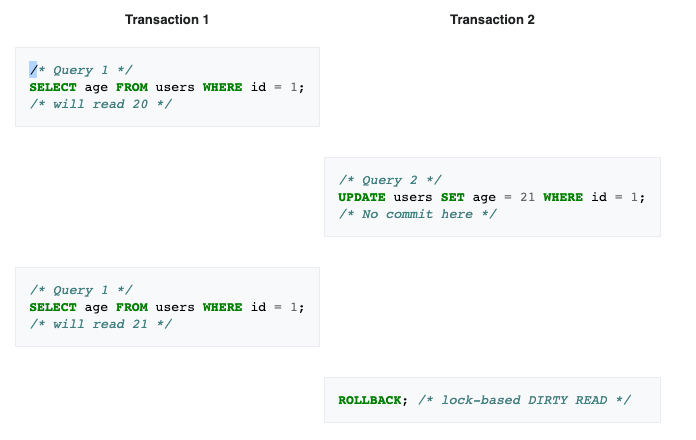
\includegraphics[width=0.7\linewidth]{images/worksheet_6_solution_1.png}
        \end{center}

        \item Non-repeatible Reads
        \begin{itemize}
            \item A non-repeatable read occurs when, during the course of a transaction,
            a row is retrieved twice and the values within the row differ between reads.
        \end{itemize}

        \begin{center}
        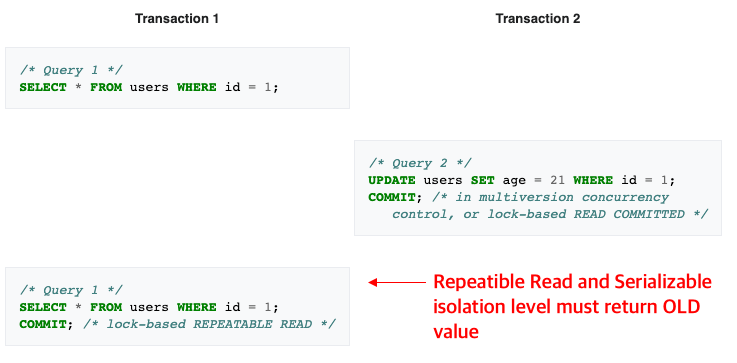
\includegraphics[width=0.7\linewidth]{images/worksheet_6_solution_2.png}
        \end{center}

        \item Phantom Reads
        \begin{itemize}
            \item A phantom read occurs when, in the course of a transaction,
            new rows are added or removed by another transaction to the records
            being read.
        \end{itemize}

        \begin{center}
        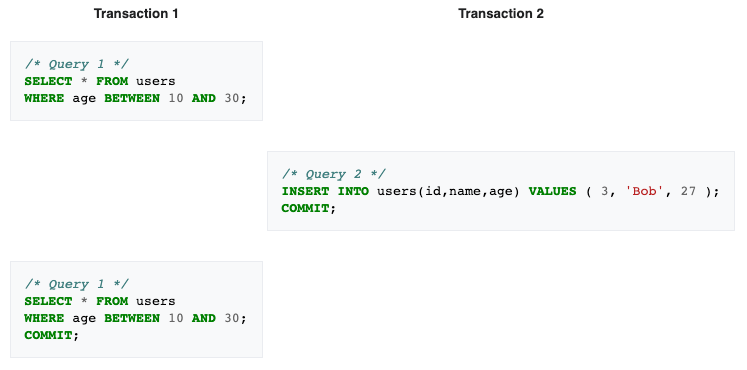
\includegraphics[width=0.7\linewidth]{images/worksheet_6_solution_3.png}
        \end{center}

        \item Isolation Levels
        \begin{itemize}
            \item SET TRANSACTION ISOLATION LEVEL READ UNCOMMITTED;
            \begin{itemize}
                \item is the lowest isolation level
                \item allows to read a transaction that's not yet committed
                \item transactions are not isolated from each other
            \end{itemize}

            \item SET TRANSACTION ISOLATION LEVEL READ COMMITTED;
            \begin{itemize}
                \item Does not allow to read a transaction that's not yet committed
                \item Prevents other transactions from reading, updating or deleting while commit
            \end{itemize}
            \item SET TRANSACTION ISOLATION LEVEL REPEATIBLE READ;
            \begin{itemize}
                \item Is the higher level of isolation
                \item Guarentees everything of READ COMMITTED level
                \item Can read unchanged data in subsequent reads
            \end{itemize}
            \item SET TRANSACTION ISOLATIO LEVEL SERIALIZABLE
            \begin{itemize}
                \item Is the highest level of isolation
                \item Guarentees everything of READ REPEATIBLE READ;
                \item No new data can be seen by a subsequent read.
            \end{itemize}

            \bigskip

            \begin{center}
            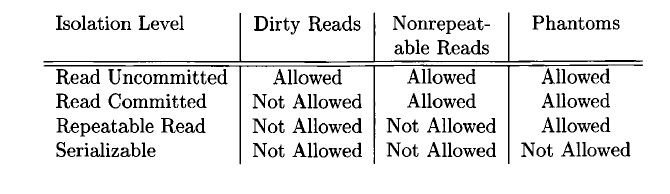
\includegraphics[width=0.7\linewidth]{images/worksheet_6_solution_4.png}
            \end{center}

            \bigskip

            \underline{\textbf{References:}}

            \begin{itemize}
                \item Stack Overflow: Difference between 'read commited' and 'repeatable read', \href{https://stackoverflow.com/questions/4034976/difference-between-read-commited-and-repeatable-read}{link}
                \item Wikipedia: Isolation (database systems), \href{https://en.wikipedia.org/wiki/Isolation_%28database_systems%29#READ_UNCOMMITTED_.28dirty_reads.29}{link}
            \end{itemize}
        \end{itemize}
    \end{itemize}

    \item \textbf{Exercise 8.1.1:}

    \bigskip

    \begin{enumerate}[a)]
        \item

    \begin{lstlisting}[language=SQL]
    CREATE VIEW RichExec AS
        SELECT * FROM MovieExec
        WHERE netWorth >= 10000000;
    \end{lstlisting}

        \bigskip

        \underline{\textbf{Notes:}}

        \bigskip

        \begin{itemize}
            \item Virtual Views
            \begin{itemize}
                \item \textbf{Syntax:} CREATE VIEW $<\text{view-name}>$ AS $<\text{view-definition}>$
                \item Contrasts to database that exists in physical storage
                \item Exists in RAM
                \item Is created using query
                \item can be used like a relation

                \bigskip

                \underline{\textbf{Notes:}}

                \bigskip

        \begin{lstlisting}[language=SQL]
        CREATE VIEW ParamountMovies AS
            SELECT title, year
            FROM Movies
            WHERE studioName = 'Paramount';
        \end{lstlisting}
            \end{itemize}
        \end{itemize}

        \item

    \begin{lstlisting}[language=SQL]
    CREATE VIEW StudioPres AS
        SELECT * FROM Movies
        INNER JOIN Studio ON cert# = presC#;
    \end{lstlisting}

        \item

    \begin{lstlisting}[language=SQL]
    CREATE VIEW ExecutiveStar AS
        SELECT * FROM MovieExec
        NATURAL JOIN MovieStar;
    \end{lstlisting}
    \end{enumerate}

    \item \textbf{Exericse 8.1.2:}

    \begin{enumerate}[a)]
        \item

    \begin{lstlisting}[language=SQL]
    SELECT name, gender FROM ExecutiveStar;
    \end{lstlisting}

        \item

    \begin{lstlisting}[language=SQL]
    SELECT name FROM RichExec WHERE netWorth > 10000000;
    \end{lstlisting}

        \item

    \begin{lstlisting}[language=SQL]
    SELECT name FROM StudioPres
    NATURAL JOIN ExecutiveStar
    WHERE netWorth > 50000000
    \end{lstlisting}
    \end{enumerate}

    \item \textbf{Exericse 8.2.1:}

    \bigskip

    \textit{RichExec} is updatable.

    \underline{\textbf{Notes:}}

    \bigskip

    \begin{itemize}
        \item Updatable View Conditions
        \begin{itemize}
            \item The WHERE cluase in CREATE VIEW must not be a subquery
            \item The FROM clause has only one occurence of R
            \item The SELECT clause must include enough attributes
            \item NOT NULL attributes must have default values
            \begin{itemize}
                \item A solution to this is by including the attribute without
                default value in CREATE VIEW
            \end{itemize}

            \bigskip

            \underline{\textbf{Example:}}

            \bigskip

    \begin{lstlisting}[language=SQL]
    Movies(title, year, length, genre, studioName, producerC#)
    Suppose studioName is NOT NULL but has no default value. Then, a fix is:

    CREATE VIEW Paramount AS
        SELECT studioName, title, year
        FROM Movies
        WHERE studioName = 'Paramount';
    \end{lstlisting}

        \end{itemize}
    \end{itemize}

    \bigskip

    \item \textbf{Exericse 8.2.2:}

    \bigskip

    \begin{enumerate}[a)]
        \item No. It is not updatable. Since,

        \begin{enumerate}[1.]
            \item studioName attribute in Movies is NOT NULL without default value
        \end{enumerate}

        \item

    \begin{lstlisting}[language=SQL]
    CREATE TRIGGER DisneyComediesInsert
    INSTEAD OF INSERT ON DisneyComedies
    REFERENCING
        NEW ROW AS NewTuple
    FOR EACH ROW
    INSERT INTO Movies(title, year, length, genre, studioName)
    VALUES(NewTuple.title, NewTuple.year, NewTuple.length, 'comedy', 'Disney');
    \end{lstlisting}

        \bigskip

        \underline{\textbf{Notes:}}

        \bigskip

        \begin{itemize}
            \item Using Trigger in VIEW
            \begin{itemize}
                \item Uses INSTEAD OF in place of BEFORE or AFTER
                \item When event causes the trigger, the trigger is done instead of the event

                \bigskip

                \underline{\textbf{Example:}}

    \begin{lstlisting}[language=SQL]
    CREATE VIEW ParamountMovies AS
        SELECT title, year
        FROM Movies
        WHERE studioName = 'paramount';

    CREATE TRIGGER ParamountInsert
    INSTEAD OF INSERT ON ParamountMovies
    REFERENCING NEW ROW AS NewRow
    FOR EACH ROW
    INSERT INTO Movies(title, year, studioName)
    VALUES(NewRow.title, NewRow.year, 'Paramount');
    \end{lstlisting}

            \end{itemize}
        \end{itemize}

        \item

    \begin{lstlisting}[language=SQL]
    CREATE TRIGGER DisneyComediesInsert
    INSTEAD OF INSERT ON DisneyComedies
    REFERENCING
        NEW ROW AS NewTuple
        OLD ROW AS OldTuple
    FOR EACH ROW
    UPDATE Movies
    SET length=NewTuple.length
    WHERE title=OldTuple.title AND year=OldTuple.year;
    \end{lstlisting}

    \end{enumerate}

    \item \textbf{Exercise 8.2.3}

    \bigskip

    \begin{enumerate}[a)]
        \item No. the view is not updatable. Because for it to be updatable,
        only one relation must exist in FROM
        \item

    \begin{lstlisting}[language=SQL]
    CREATE TRIGGER NewPCInsert
    INSTEAD OF INSERT ON NewPC
    REFERENCING
        NEW ROW AS NewTuple
        OLD ROW AS OldTuple
    FOR EACH ROW
    INSERT INTO PC(model speed, ram, hd ,price)
    VALUES (NewTuple.model, NewTuple.speed, NewTuple.ram, NewTuple.hd, NewTuple.price);

    INSERT INTO Product(maker, model, type)
    VALUES (NewTuple.maker, NewTuple.model, 'pc');
    \end{lstlisting}

        \item

    \begin{lstlisting}[language=SQL]
    CREATE TRIGGER NewPCUpdate
    INSTEAD OF INSERT ON NewPC
    REFERENCING
        NEW ROW AS NewTuple
    FOR EACH ROW
    UPDATE PC
    SET model=NewTuple.model
        speed=NewTuple.speed,
        ram=NewTuple.ram,
        hd=NewTuple.hd,
        price=NewTuple.price;

    UPDATE Product
    SET maker=NewTuple.maker,
        model=NewTuple.model,
        type='pc';
    \end{lstlisting}

        \bigskip

        \begin{mdframed}
            \underline{\textbf{Correct Solution:}}

    \begin{lstlisting}[language=SQL]
    CREATE TRIGGER NewPCUpdate
    INSTEAD OF UPDATE ON NewPC
    REFERENCING
        NEW ROW AS NewTuple
    FOR EACH ROW
    UPDATE PC
    SET model=NewTuple.model
        speed=NewTuple.speed,
        ram=NewTuple.ram,
        hd=NewTuple.hd,
        price=NewTuple.price;

    UPDATE Product
    SET maker=NewTuple.maker,
        model=NewTuple.model,
        type='pc';
    \end{lstlisting}
        \end{mdframed}

        \item

    \begin{lstlisting}[language=SQL]
    CREATE TRIGGER NewPCDelete
    INSTEAD OF DELETE ON NewPC
    REFERENCING
        NEW ROW AS NewTuple
    FOR EACH ROW
    DELETE FROM PC
    WHERE model=NewTuple.model;

    DELETE FROM Product
    WHERE model=NewTuple.model;
    \end{lstlisting}

    \end{enumerate}

    \item

    \begin{enumerate}[a)]
        \item

    \begin{lstlisting}[language=SQL]
    CREATE INDEX studioNameIndex Studio(name)
    \end{lstlisting}

        \bigskip

        \underline{\textbf{Notes:}}

        \bigskip

        \begin{itemize}
            \item Indexes
            \begin{itemize}
                \item \textbf{Syntax (Create Index):}

                CREATE INDEX $<\text{index-name}>$ $R(<\text{attributes}>)$
                \item \textbf{Syntax (Drop Index):}

                DROP INDEX $<\text{index-name}>$
                \item Used to find tuples in a very large database
                \begin{itemize}
                    \item Is efficient
                \end{itemize}
                \item Can be thought as (key, value) pair in a binary search tree
                \item e.g. Declaring Index

    \begin{lstlisting}[language=SQL]
    CREATE INDEX KeyIndex ON Movies(title, year);
    \end{lstlisting}

                \item e.g. Dropping index

    \begin{lstlisting}[language=SQL]
    CREATE INDEX KeyIndex ON Movies(title, year);
    \end{lstlisting}

            \end{itemize}
        \end{itemize}

        \item

    \begin{lstlisting}[language=SQL]
    CREATE INDEX movieExecAddressIndex MovieExec(address)
    \end{lstlisting}

        \item

    \begin{lstlisting}[language=SQL]
    CREATE INDEX movieKeyIndex Movies(genre, length)
    \end{lstlisting}

    \end{enumerate}

    \item \textbf{Exercise 8.4.1:}

    \bigskip

    \begin{tabular}{c|cccc}
        Action & No Index & Star Index & Movie Index & Both Indexes\\
        \hline
        $Q_1$ & 100 & 4 & 100 & 4\\
        \hline
        $Q_2$ & 100 & 100 & 4 & 4\\
        \hline
        $I$ & 2 & 4 & 4 & 6\\
        \hline
        Average & $2 + 100p_1 + 100p_2$ & $4 + 96p_2$ & $4 + 96p_1$ & $6 - 2p_1 - 2p_2$\\
    \end{tabular}

    \bigskip

    \underline{\textbf{Notes:}}

    \bigskip

    \begin{itemize}
        \item Database Tuning
        \begin{itemize}
            \item Index sppeds up queries that can use it
            \item Index should NOT be created when modifications are the frequent
            choice of action
        \end{itemize}
    \end{itemize}

    \item \textbf{Exercise 8.4.2:}

    Omitted for the time being

    \item \textbf{Exercise 8.5.1:}

    \bigskip

    \begin{lstlisting}[language=SQL]
    UPDATE MovieProd
    SET name='New Name'
    WHERE (title, year) IN
    (
        SELECT title, year FROM Movies
        INNER JOIN MovieExecs
        ON Movies.productC# = MovieExec.cert#
        WHERE cert# = '4567'
    );
    \end{lstlisting}

    \bigskip

    \underline{\textbf{Notes:}}

    \bigskip

    \begin{itemize}
        \item Materialized Views
        \begin{itemize}
            \item Is also known as a summary
            \item Is also known as black-box abstraction
            \item Stores view in physical storage
            \item Useful when storing expensive operation like AVG or COUNT
        \end{itemize}
    \end{itemize}
    \item \textbf{Exercise 8.5.3}

    \bigskip

    The following modifications to base tables require the modification of the
    materialized view

    \begin{itemize}
        \item PC: Updates(model, speed, ram, hd, price), Delete
        \item Product: Updates(maker, model, type), Delete
    \end{itemize}

    \bigskip

    Implementing modifications

    \begin{itemize}
        \item Updates

    \begin{lstlisting}[language=SQL]
    UPDATE NewPC
    SET maker='new-maker'
        model='new-model-number'
        speed='new-speed'
        ram='new-ram'
        hd='new-hd'
        price='new-price'
    WHERE model = 'old-model-number';
    \end{lstlisting}

        \item Delete

    \begin{lstlisting}[language=SQL]
    DELETE FROM NewPC WHERE model = 'old-model-number'
    \end{lstlisting}
    \end{itemize}

    \underline{\textbf{Notes:}}

    \begin{itemize}
        \item Materialized view of NewPC

    \begin{lstlisting}[language=SQL]
    CREATE MATIERLIZED VIEW NewPC AS
        SELECT maker, model, speed, ram, hd, price
        FROM Product, PC
        WHERE Product.model = PC.model AND type = 'pc';
    \end{lstlisting}

    \end{itemize}

    \item \textbf{Exercise 8.5.3}

    The following modifications to base tables require the modification of the
    materialized view

    \begin{itemize}
        \item Classes: Insert, Updates(class, country, displacement), Delete
        \item Ships: Insert, Updates(class), Delete
    \end{itemize}

    \begin{itemize}
        \item Insert

    \begin{lstlisting}[language=SQL]
    INSERT INTO ShipStats
    VALUES (
        SELECT country, AVG(displacement), COUNT(*)
        FROM Classes, Ships
        WHERE Classes.class = ships.class
        GROUP BY country
        HAVING country='name-of-country'
    )
    \end{lstlisting}

        \item Updates

    \begin{lstlisting}[language=SQL]
    DELETE FROM ShipStats WHERE country = 'name-of-country';
    INSERT INTO ShipStats
    VALUES (
        SELECT country, AVG(displacement), COUNT(*)
        FROM Classes, Ships
        WHERE Classes.class = ships.class
        GROUP BY country
        HAVING country='name-of-country'
    )
    \end{lstlisting}

        \item Delete

    \begin{lstlisting}[language=SQL]
    DELETE FROM ShipStats WHERE country = 'country'
    \end{lstlisting}

    \end{itemize}

    \item \textbf{Exercise 8.5.4}

    \bigskip

    \underline{\textbf{Notes:}}

    \bigskip

    \begin{itemize}
        \item Rewriting Queries to use Materialized View
        \begin{itemize}
            \item Conditions under which we can replace part of the query Q by the
            view V
            \begin{enumerate}
                \item The relations in list $R_v$ all appear in the list $R_Q$
                \item The condition $C_Q$ is equivalent to $C_V$ AND $C$ for some
                condition $C$. As a special case, $C_Q$ could be equivalent to $C_V$,
                in which case the "AND $C$" is unnecessary.
            \end{enumerate}
            \item Once the conditions are met, $Q$ can be re-written to $V$ as follows
            \begin{itemize}
                \item Replace the list $R_Q$ by $V$ and the relations that are on list $R_Q$
                but not on $R_V$
                \item Replace $C_Q$ by $C$. If $C$ is not needed (i.e. $C_V = C_Q$), then
                there is no WHERE clause
            \end{itemize}
        \end{itemize}
    \end{itemize}

\end{enumerate}

\end{document}